\section{Outlook}
\begin{frame}{Outlook}
\begin{itemize}
\item inclusive distributions: $\DeriveF{{p_{T,\PaQ}}}{g_1},\DeriveF{{y_{\PaQ}}}{g_1}, \ldots$ \iRef{Laenen,Riemersma,Smith,van Neerven}
\item correlated distributions: $\DeriveF{{M_{\PQ\PaQ}^2}}{g_1}, \DeriveF{\phi_{\PQ\PaQ}}{g_1}, \text{TMD}, \ldots$ \iRef{Harris,Smith}
\item<2-> full neutral current (NC) contributions: $F_3^{\PZ\Pgg}, g_4^{\PZ\Pgg}, g_5^{\PZ\Pgg}$ and $F_2^{\PZ}, F_L^{\PZ}, g_1^{\PZ}$
\item<2-> distributions of full NC structure functions: $\DeriveF{p_{T,\PaQ}}{g_1^{NC}},\DeriveF{{M_{\PQ\PaQ}^2}}{g_1^{NC}}, \ldots$
\end{itemize}

\uncover<3->{\vspace{1cm}
\setbeamercolor{thanks}{bg=UniRot,fg=white}
\begin{beamercolorbox}[ht=2.5ex,dp=1ex,center]{thanks}
Thank you for your attention!
\end{beamercolorbox}}
\end{frame}

\section*{Backup}

\begin{frame}{Backup: Partonic Results - Gluon Channel}
\begin{align*}
%2xF_1(x) &\sim \xi g(\xi) \otimes \left(c_{T,\Pg}^{(0)} + 4\pi\alpha_s\left[c_{T,\Pg}^{(1)} + \ln\left(\frac{\mu^2}{m^2}\right)\bar c_{T,\Pg}^{(1)}\right]\right)\\
g_1 &\sim \alpha_s\cdot\Delta \Pg \otimes \left(c_{P,\Pg}^{(0)} + 4\pi\alpha_s\left[c_{P,\Pg}^{(1)} + \ln\left(\frac{\mu^2}{m^2}\right)\bar c_{P,\Pg}^{(1)}\right]\right)
\end{align*}
\begin{center}
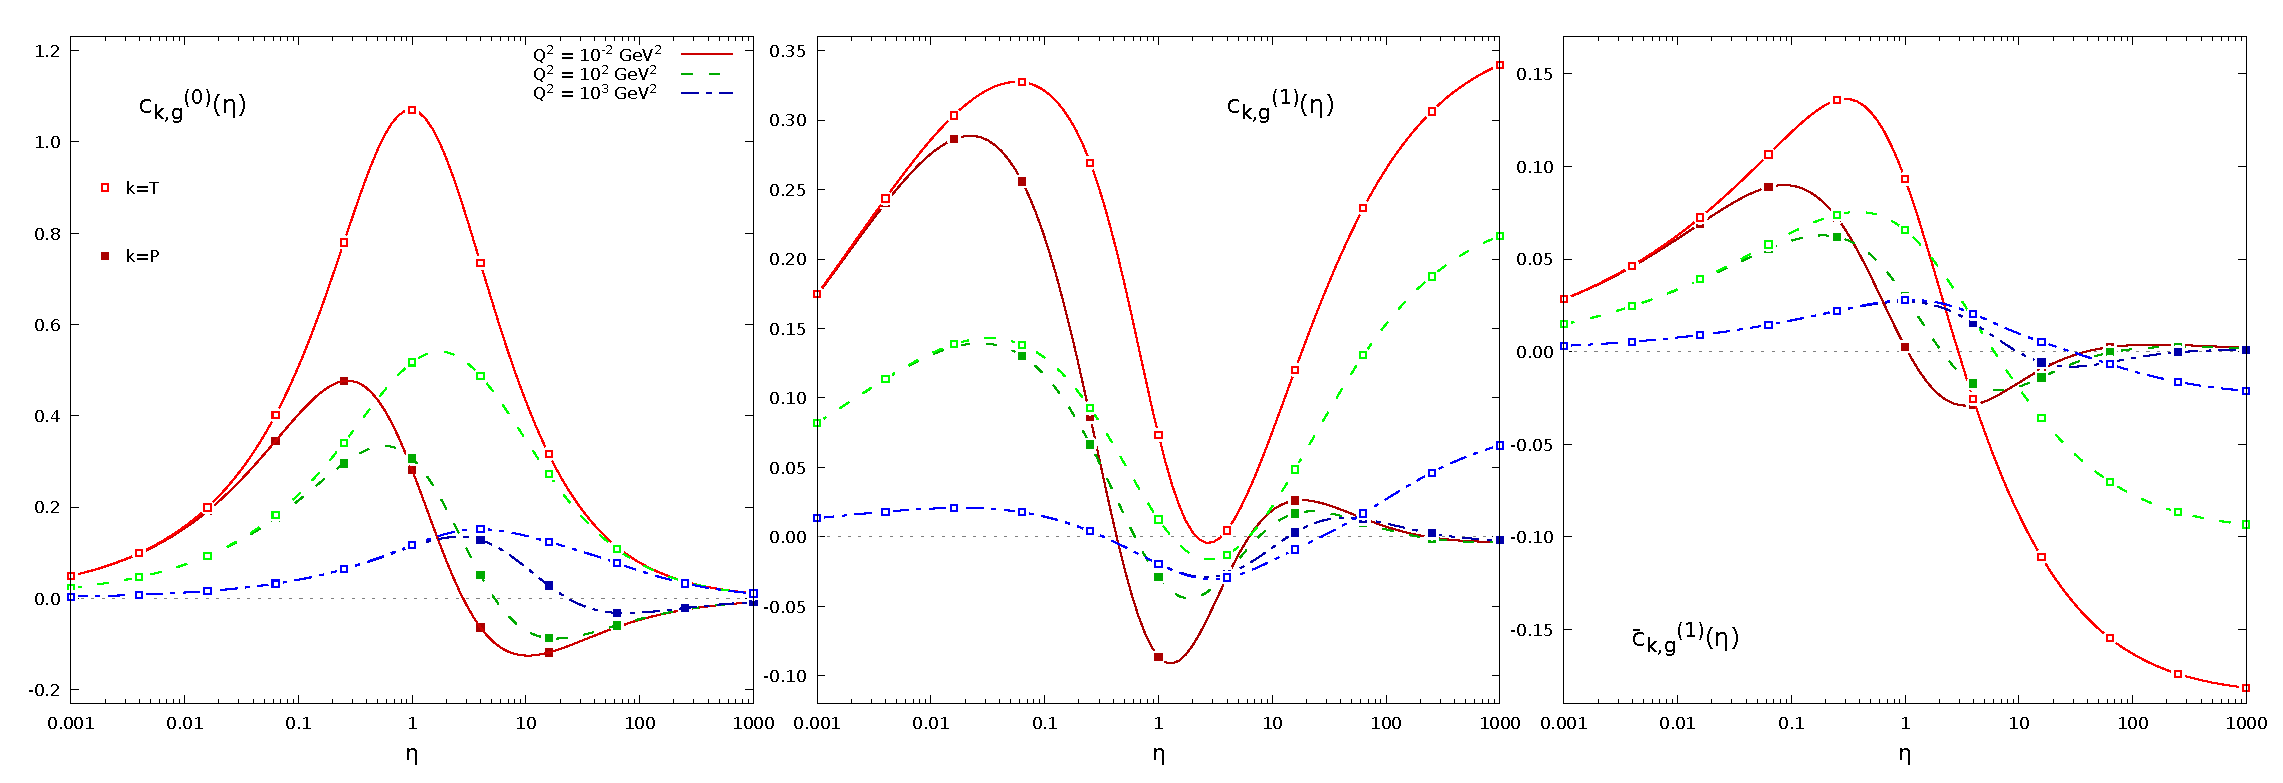
\includegraphics[width=\textwidth]{img/cgTP}
\end{center}
\[\eta = \frac{s-4m^2}{4m^2},\quad m=m_b=\SI{4.75}{\GeV}\]
\end{frame}

\begin{frame}{Backup: Partonic Results - Light Quark Channel}
\begin{align*}
g_1 &\sim {\color{red}\alpha_s^2}\sum_{q}\left(\Delta \Pq+\Delta \Paq\right) \otimes \left(e_H^2\left[c_{P,\Pq}^{(1)} + \ln\left(\frac{\mu^2}{m^2}\right)\bar c_{P,\Pq}^{(1)}\right] + e_q^2 d_{P,\Pq}^{(1)}\right)
\end{align*}
\begin{center}
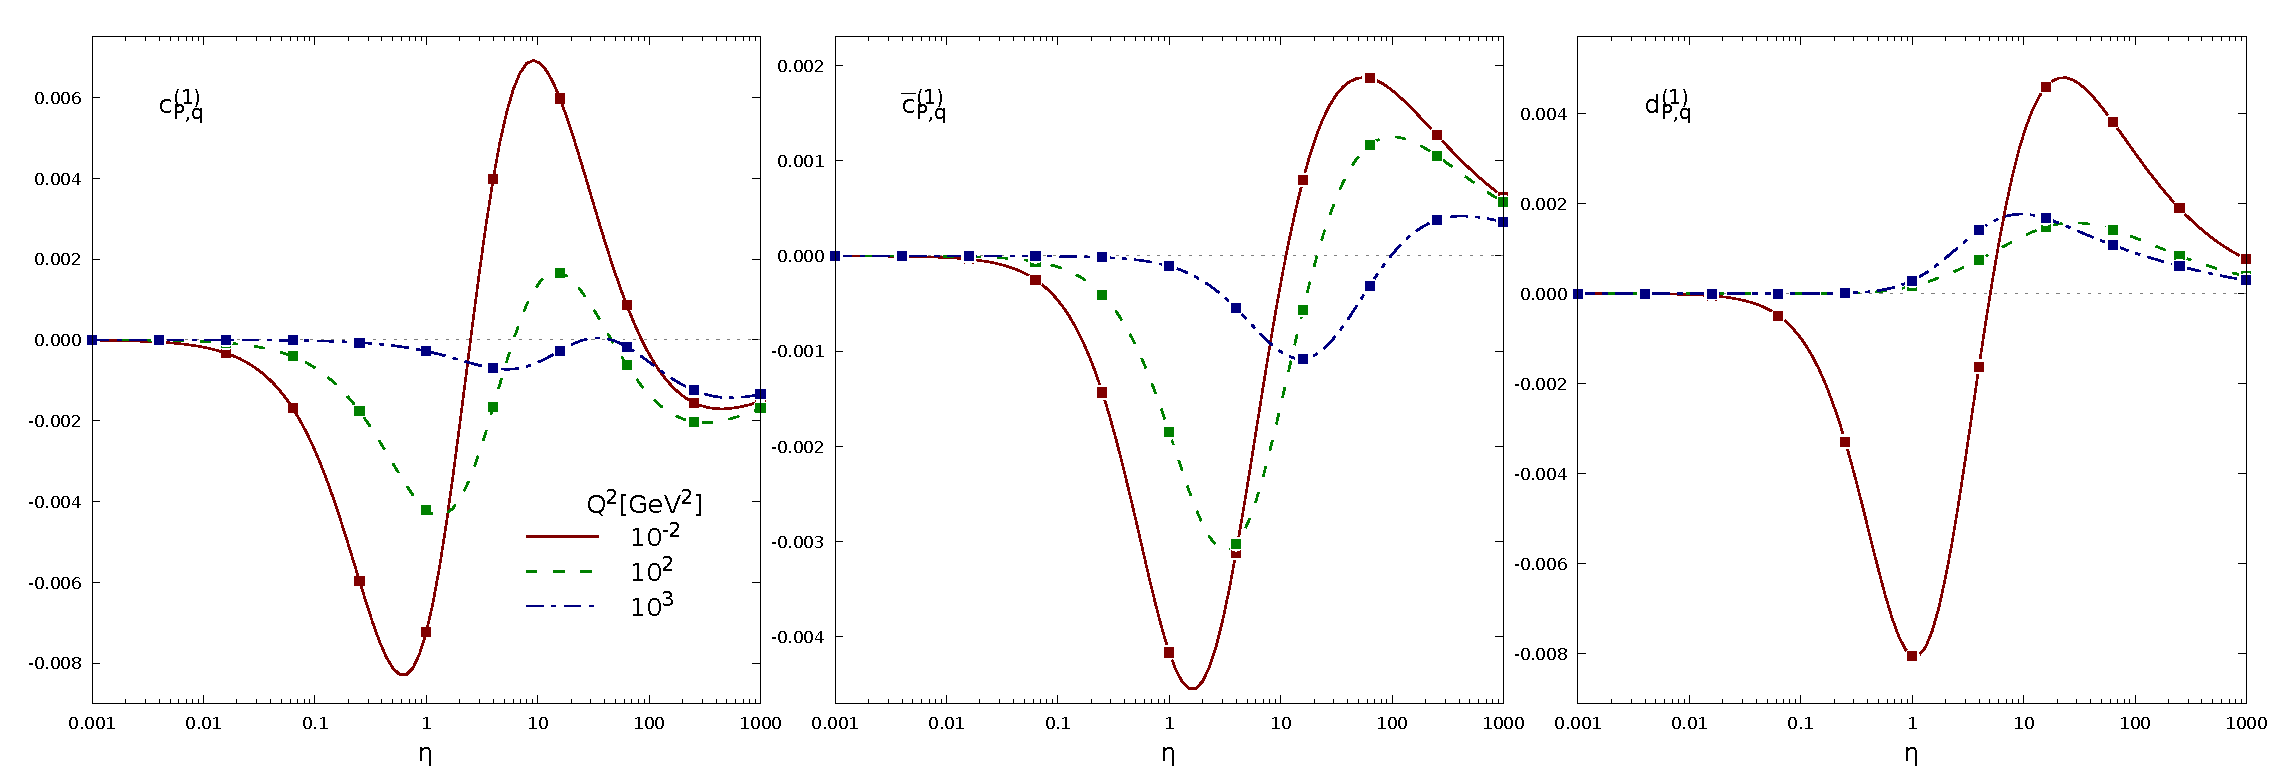
\includegraphics[width=\textwidth]{img/cdqP}
\end{center}
\[\eta = \frac{s-4m^2}{4m^2},\quad m=m_b=\SI{4.75}{\GeV}\]
\end{frame}


\begin{frame}{Backup: Hadronic Results - PDF Uncertainties DSSV}
\newcolumntype{w}{>{\centering\arraybackslash} m{.65\linewidth} }
\newcolumntype{n}{>{\centering\arraybackslash} m{.35\linewidth} }
\begin{tabular}{wn}
\begin{center}
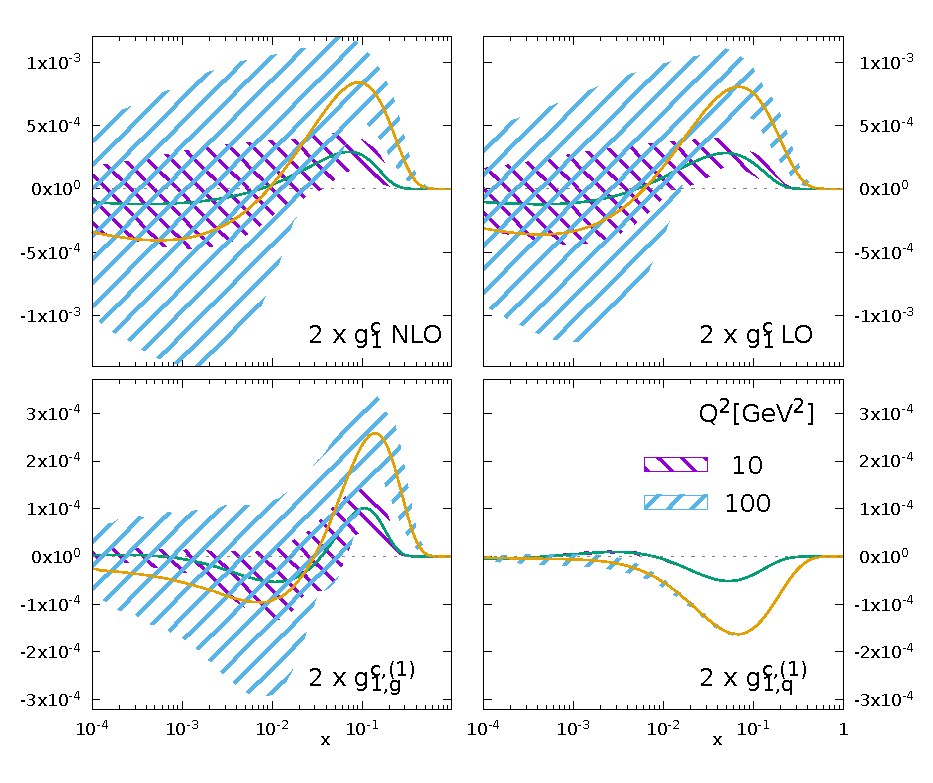
\includegraphics[height=.95\textheight]{img/g1Parts-pdf}
\end{center} & 
\begin{itemize}
\item gluon dominates
\item sign uncontrained
\item quark band small
\item default gluon is small
\end{itemize}
\end{tabular}
\end{frame}

\begin{frame}{Backup: Hadronic Results - Mass Variation}
\begin{center}
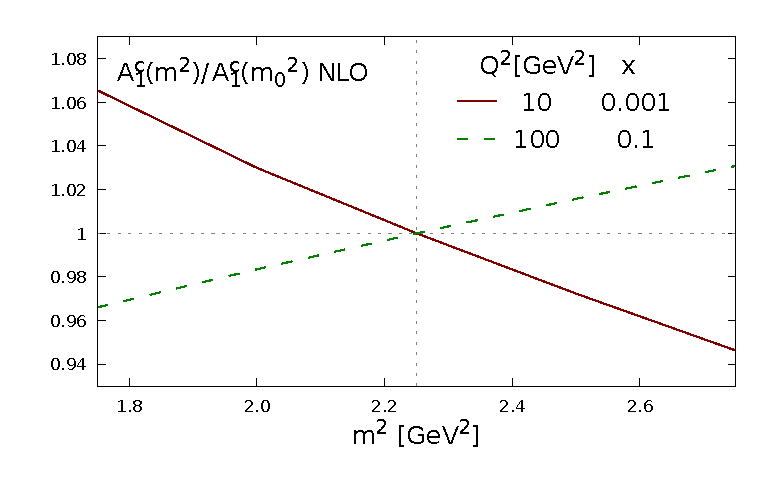
\includegraphics[width=.75\textwidth]{img/A1-m2}
\end{center}
\[m_0=\SI{1.5}{\GeV}\]
\end{frame}
